\documentclass[11pt,a4paper]{article}
\usepackage[utf8]{inputenc}
\usepackage[T1]{fontenc}
\usepackage{amsmath, amssymb, amsthm}
\usepackage{graphicx}
\usepackage{hyperref}
\usepackage{booktabs}
\usepackage{bm}
\usepackage{geometry}
\usepackage{natbib}
\usepackage{algorithm}
\usepackage{algpseudocode}
\usepackage{xcolor}
\usepackage{listings}
\usepackage{multirow}
\usepackage{array}
\usepackage{enumitem}
\usepackage{parskip}
\usepackage{tikz}
\usetikzlibrary{shapes.geometric,arrows.meta,positioning,fit,backgrounds,calc}

\geometry{margin=1in, top=0.9in, bottom=0.9in}

% NeurIPS-style: tighter spacing
\setlength{\parskip}{3pt}

\definecolor{codeblue}{RGB}{30,100,200}
\definecolor{layerA}{RGB}{210,230,255}
\definecolor{layerB}{RGB}{210,255,220}
\definecolor{layerC}{RGB}{245,220,255}
\definecolor{layerD}{RGB}{255,235,210}
\lstset{
  basicstyle=\ttfamily\small,
  keywordstyle=\color{codeblue}\bfseries,
  commentstyle=\color{gray},
  breaklines=true,
  frame=single
}

\newtheorem{definition}{Definition}
\newtheorem{proposition}{Proposition}
\newtheorem{remark}{Remark}

% -----------------------------------------------------------------------
\title{\textbf{Two Brains, One Network: Dual-Process Topology Management\\for Heterogeneous Physics-Informed Kolmogorov-Arnold Networks}}
\author{OpKAN Engineering Team \\ \texttt{github.com/RicardoLaMo/OpKAN}}
\date{March 2026}

\begin{document}
\maketitle

% -----------------------------------------------------------------------
\begin{abstract}
Kolmogorov-Arnold Networks (KANs) place learnable activation functions on edges,
enabling surgical symbolic replacement of individual edges at runtime. This
introduces a class of management problem that gradient descent cannot solve:
\emph{topology parameterization selection} --- deciding when to convert a B-spline
edge to a symbolic form, when to prune it, and what symbolic formula preserves the
network's mathematical invariants. We identify five chronic failure modes of
heterogeneous KAN topology (B-spline $\cup$ symbolic) and show they decompose
naturally across two cognitive timescales. We present a \textbf{dual-process topology
agent}: System~1 (7B model, $<$50\,ms) handles high-frequency reflexive maintenance
--- pruning near-zero edges, adjusting learning rates; System~2 (32B model, 200--500\,ms)
handles low-frequency strategic surgery --- symbolic edge replacement guided by PDE
geometry and market regime signals. A typed DSL with static AST allowlist and atomic
rollback guarantees type safety, vocabulary restriction, and transactional integrity
for every mutation. Demonstrated on a physics-informed KAN solving the Heston PDE:
all five financial monotonicity checks pass \emph{only} under dual-process control ---
not from PDE training alone --- establishing training objective insufficiency as a
general failure mode in physics-constrained networks under distributional shift.
Sustained throughput reaches 26,300\,smp/sec on H200 with zero GPU blocking.
\end{abstract}

% =====================================================================
\section{Introduction}
\label{sec:intro}
% =====================================================================

\subsection{The Topology Surgery Problem in Heterogeneous KANs}
\label{sec:intro:surgery}

A KAN with a mixed topology --- some edges parameterized as B-splines, others replaced
with closed-form symbolic functions (\texttt{C2SymbolicEdge}), others pruned to zero
(\texttt{ZeroEdge}) --- is a qualitatively different computational object from a
homogeneous MLP. The edge-level parameterization choice is not a hyperparameter set
before training: it is an ongoing decision made during training as the network's
activation profiles evolve, regime signals change, and new domain knowledge becomes
available.

Gradient descent cannot make this decision. It can optimize the coefficients of a
B-spline edge but has no mechanism to decide that the edge's activation profile now
closely approximates $e^{-|x|}$ and should be replaced with a closed-form symbolic
function. It can drive a B-spline's coefficients toward zero but provides no pruning
signal because the gradient of a near-zero activation is also near-zero. This is the
\emph{topology surgery problem}: a class of decisions about the network's structure
that falls strictly outside the scope of gradient-based optimization.

This problem manifests in five distinct chronic failure modes of heterogeneous KAN
topology management:

\begin{enumerate}[nosep]
  \item \textbf{Topology stagnation.} Near-zero B-spline edges persist through training
  because their loss gradient is also near-zero. The edge contributes nothing but
  continues consuming computation.

  \item \textbf{Parameterization lock-in.} Gradient descent never has incentive to
  change an edge's parameterization class. A B-spline that closely approximates
  $\sin(x)$ remains a B-spline indefinitely, losing both interpretability and
  efficiency.

  \item \textbf{Symbolic-numerical tension.} Symbolic edges have no trainable
  parameters. In a mixed topology, gradient cannot flow through symbolic edges to
  inform neighboring B-spline adaptations --- creating dead zones in the optimization
  landscape.

  \item \textbf{Regime blindness.} Under distributional shift (market regime change),
  a frozen topology cannot adapt. Weight updates shift the learned function but cannot
  restructure which edges carry which mathematical primitives.

  \item \textbf{$C^2$ instability.} Under aggressive learning rates, B-spline
  coefficient updates can push activation profiles into configurations that are
  technically $C^2$ but produce numerically ill-conditioned second derivatives ---
  critical in PDE settings where cross-derivatives are explicitly evaluated.
\end{enumerate}

\subsection{Why Two Brains}
\label{sec:intro:twobrains}

The five problems decompose naturally by frequency and cognitive type. Problems~1
and~5 (stagnation and $C^2$ instability) are \textbf{high-frequency, low-complexity}:
they can be detected from local statistics (L1 norm of edge activations,
second-derivative magnitude) and resolved with simple actions (prune, adjust lr).
A fast model ($<$50\,ms, 7B parameters) is sufficient --- the decision requires
pattern recognition, not mathematical reasoning.

Problems~2, 3, and~4 (parameterization lock-in, symbolic-numerical tension, regime
blindness) are \textbf{low-frequency, high-complexity}: they require reasoning about
the network's global activation geometry, the mathematical properties of candidate
symbolic functions, and the relationship between regime signals and structural
adaptation. A slow, large model (200--500\,ms, 32B parameters) is necessary --- the
decision requires chain-of-thought reasoning over PDE structure.

One brain of either type cannot address all five. A single fast model makes
mathematically incoherent symbolic replacements. A single slow model blocks the GPU.
The dual-process design is not an engineering compromise --- it is a consequence of
the cognitive structure of the topology surgery problem.

\subsection{Contributions}
\label{sec:intro:contributions}

\begin{enumerate}
  \item A taxonomy of five chronic management problems in heterogeneous KAN topology,
  and a demonstration that they decompose across two cognitive timescales.

  \item A \textbf{dual-process topology agent} (System~1/System~2) that addresses all
  five, with the two paths operating concurrently without GPU blocking.

  \item A \textbf{typed DSL} with AST allowlist and atomic rollback providing type
  safety, vocabulary restriction ($C^2$ continuity preserved by construction), and
  transactional integrity.

  \item \textbf{Evaluation on Heston options pricing} --- a testbed where $C^2$
  continuity, PDE geometry reasoning, and real-time regime adaptation impose hard
  correctness requirements that expose dual-process advantages invisible in
  unconstrained settings.

  \item The \textbf{training objective insufficiency finding}: PDE residual
  minimization alone does not produce regime-ordered behavior under distributional
  shift --- a result that generalizes beyond options pricing.
\end{enumerate}

\subsection{Paper Organization}

Section~\ref{sec:related} situates the work in the literature.
Section~\ref{sec:background} develops the heterogeneous KAN background and the Heston
testbed. Section~\ref{sec:agent} presents the dual-process topology agent.
Section~\ref{sec:regime} describes the market regime conditioning layer.
Section~\ref{sec:experiments} presents experimental evaluation.
Section~\ref{sec:discussion} provides discussion and addresses the distinction from
LangChain-style systems. Section~\ref{sec:conclusion} concludes.

% =====================================================================
\section{Related Work}
\label{sec:related}
% =====================================================================

\subsection{KANs and Symbolic Regression}

The KAN architecture \citep{liu_etal_2024_kan} places learnable activation functions
on edges rather than nodes, enabling edge-level interpretability and surgical symbolic
replacement. The theoretical foundation is Kolmogorov's superposition theorem
\citep{kolmogorov1957representation}. MonoKAN \citep{polo_molina_etal_2024_monokan}
extends KANs with certified monotonicity constraints. Symbolic edge replacement is
available in the original KAN library but is \emph{manual and offline}. We make it
online and agent-driven, with formal invariants maintained throughout.

\subsection{Physics-Informed Learning}

PINNs \citep{raissi2019physics} convert a PDE boundary value problem into an
unconstrained optimization by embedding the differential operator residual in the
loss. Financial applications \citep{horvath2021deep} have generally used standard MLP
backbones; the $C^2$ continuity requirement of the Heston cross-derivative term has
received limited attention. Deep hedging \citep{buhler2019deep} and Neural SDEs
\citep{kidger2021neural} extend the neural approach to replication and continuous-time
dynamics, but do not enforce specific boundary conditions in the Heston sense.

\subsection{Neural Architecture Search}

NAS \citep{elsken2019neural} automates topology discovery through gradient-based
\citep{liu2019darts} or evolutionary search. NAS operates \emph{offline}: it finds
a fixed architecture before training begins. The dual-process agent operates
\emph{online}, on a running network, with natural language input and domain-specific
mathematical constraints. The two approaches are complementary --- NAS for
initialization, dual-process for runtime adaptation --- rather than competitive.

\subsection{Dual-Process AI and LLM Agents}

Kahneman's framework \citep{kahneman2011thinking} applied to AI agents. Toolformer
\citep{schick_etal_2023_toolformer} and ReAct \citep{yao_etal_2023_react} use LLMs
as tool orchestrators, producing text outputs over stateless API calls. The critical
distinction from these systems and from workflow frameworks (LangChain-style tool
routing) is developed in Section~\ref{sec:discussion:notlangchain}: those systems
route stateless text between API endpoints and have no persistent mathematical state
to maintain. Our agent modifies the internal mathematical structure of a running
network under formal invariants --- a fundamentally different task.

% =====================================================================
\section{Background: Heterogeneous KAN Topology}
\label{sec:background}
% =====================================================================

\subsection{KAN Edge Activations}
\label{sec:background:edges}

The Kolmogorov-Arnold representation theorem \citep{kolmogorov1957representation}
guarantees that any continuous function can be expressed as a composition of
univariate functions. The KAN architecture \citep{liu_etal_2024_kan} operationalizes
this by placing learnable activation functions on \emph{edges} rather than nodes.
Each edge is implemented as a \texttt{BSplineEdge} module. The basis functions are
defined by the Cox--de Boor recursion over a knot sequence $\mathbf{t}$:
\begin{align}
B_{i,0}(x) &= \mathbf{1}[t_i \leq x < t_{i+1}] \label{eq:cox_de_boor_1} \\
B_{i,k}(x) &= \frac{x - t_i}{t_{i+k} - t_i} B_{i,k-1}(x)
             + \frac{t_{i+k+1} - x}{t_{i+k+1} - t_{i+1}} B_{i+1,k-1}(x)
\label{eq:cox_de_boor_2}
\end{align}
OpKAN uses $G=5$ interior intervals and spline order $k=3$ (cubic), giving $G+k=8$
basis functions per edge. The edge activation combines a SiLU base with a trained
spline correction:
\begin{equation}
\phi(x) = w_\text{base} \cdot \text{SiLU}(x)
         + w_\text{spline} \cdot \sum_{i=1}^{8} c_i B_{i,3}(x)
\label{eq:bspline_edge}
\end{equation}
where $w_\text{base}, w_\text{spline} \in \mathbb{R}$ and $\{c_i\}_{i=1}^8$ are
trainable. Because each $B_{i,3}$ is $C^2$ by construction, Eq.~\eqref{eq:bspline_edge}
is $C^2$ for any choice of coefficients.

The PI-KAN uses a $[3, 16, 1]$ configuration (inputs $(S,v,t)$, 16-node hidden layer,
scalar output $V$). The forward pass aggregates edge outputs by summation:
\begin{equation}
h_j^{(\ell)} = \sum_{i=1}^{n_\text{in}^{(\ell)}} \phi_{ij}^{(\ell)}\!\left(h_i^{(\ell-1)}\right)
\label{eq:kan_forward}
\end{equation}

\subsection{Heterogeneous Edge Types}
\label{sec:background:heterogeneous}

Three edge types coexist in OpKAN at runtime:
\begin{itemize}[nosep]
  \item \texttt{BSplineEdge}: 8 basis functions, trainable coefficients $+$ SiLU base.
  \item \texttt{C2SymbolicEdge}: closed-form expression from the 20-function AST
  allowlist, no trainable parameters.
  \item \texttt{ZeroEdge}: returns \texttt{torch.zeros\_like(x)} --- correct PRUNE
  semantics (not \texttt{nn.Sequential()} which is identity).
\end{itemize}

The topology at any training step is a mix of these types. This heterogeneity enables
interpretability and efficiency gains --- and creates the five chronic problems
identified in Section~\ref{sec:intro:surgery}.

\subsection{The Heston PDE Testbed}
\label{sec:background:heston}

The Heston stochastic volatility model \citep{heston1993closed} describes risk-neutral
dynamics for spot price $S_t$ and variance $v_t$:
$dS_t = r S_t \, dt + \sqrt{v_t} S_t \, dW_t^S$, $\;dv_t = \kappa(\theta - v_t) \, dt + \sigma \sqrt{v_t} \, dW_t^v$,
where $\text{Corr}(dW^S, dW^v) = \rho \, dt$. By It\^o's lemma, option fair value
$V(S,v,t)$ satisfies the Heston PDE:
\begin{equation}
\frac{\partial V}{\partial t}
+ \frac{1}{2}vS^2\frac{\partial^2 V}{\partial S^2}
+ \rho\sigma vS\frac{\partial^2 V}{\partial S\partial v}
+ \frac{1}{2}\sigma^2 v\frac{\partial^2 V}{{\partial v}^2}
+ rS\frac{\partial V}{\partial S}
+ \kappa(\theta-v)\frac{\partial V}{\partial v}
- rV = 0
\label{eq:heston_pde}
\end{equation}
with boundary conditions:
$V(S, v, T) = \max(S - K, 0)$ (terminal payoff),
$V(0, v, t) = 0$ (zero spot), and
$V(S, v, t) \approx S - Ke^{-r(T-t)}$ as $S \to \infty$.

The cross-derivative term $\rho\sigma vS \,\partial^2 V / \partial S \partial v$ is
the key constraint: evaluating it via automatic differentiation requires $C^2$
continuous activations. Standard MLP architectures with ReLU activations produce
zero second derivatives, making this term numerically degenerate.

This testbed is demanding for the dual-process agent along three axes: (1) the $C^2$
continuity requirement is a hard mathematical invariant that every topology mutation
must preserve; (2) PDE geometry reasoning constrains which symbolic functions are
mathematically coherent replacements; and (3) real-time regime adaptation requires
the agent to reason about distributional shift.

\subsection{Training Objective}
\label{sec:background:loss}

Training minimizes a composite physics-informed loss:
\begin{equation}
\mathcal{L} = \underbrace{\mathbb{E}_{\bm{x} \sim \Omega}\!\left[\left|\mathcal{N}[V](\bm{x})\right|^2\right]}_{\mathcal{L}_\text{PDE}}
+ \lambda_\text{BC}\underbrace{\mathbb{E}_{\bm{x} \sim \partial\Omega}\!\left[\left|V(\bm{x}) - V_\text{target}(\bm{x})\right|^2\right]}_{\mathcal{L}_\text{BC}}
\label{eq:loss}
\end{equation}
where $\mathcal{N}[V]$ is the Heston differential operator evaluated via
\texttt{torch.autograd} with \texttt{create\_graph=True}. Collocation points
$\bm{x}=(S,v,t)$ are drawn uniformly from $[0,200]\times[0,0.5]\times[0,1]$.
This objective is necessary but \emph{not sufficient} for regime-ordered behavior ---
the key finding established in Section~\ref{sec:experiments}.

% =====================================================================
\section{Dual-Process Topology Agent}
\label{sec:agent}
% =====================================================================

\subsection{Decomposition by Cognitive Type}
\label{sec:agent:decomposition}

The five chronic problems map to two cognitive timescales as shown in
Table~\ref{tab:decomposition}. The fast path (System~1) addresses problems that can
be diagnosed from local statistics and resolved with simple actions. The slow path
(System~2) addresses problems that require multi-step mathematical reasoning over the
global network structure.

\begin{table}[ht]
\centering
\caption{Decomposition of the five chronic topology management problems by cognitive
timescale. System~1 actions are statistical threshold decisions; System~2 actions
require chain-of-thought reasoning over PDE geometry.}
\begin{tabular}{@{}llll@{}}
\toprule
Problem & System & Reasoning Type & Action \\
\midrule
Topology stagnation & 1 & Statistical threshold & PRUNE edge \\
$C^2$ instability & 1 & Magnitude monitoring & Adjust lr \\
Parameterization lock-in & 2 & Mathematical reasoning & REPLACE with symbolic \\
Symbolic-numerical tension & 2 & Global graph reasoning & Selective REPLACE/KEEP \\
Regime blindness & 2 & Regime analysis $+$ PDE & Structural adaptation \\
\bottomrule
\end{tabular}
\label{tab:decomposition}
\end{table}

\subsection{System 1 --- Reflexive Maintenance}
\label{sec:agent:sys1}

Every 10 training steps, the training loop places (step index, per-edge L1 norms,
recent loss delta) into a bounded queue (\texttt{maxsize=1}, latest-context-only).
A background thread dequeues and invokes a 7B Qwen 2.5 model, which produces a
\texttt{ReflexDecision}:

\begin{lstlisting}[language=Python]
class ReflexDecision(BaseModel):
    reasoning: str          # brief justification
    prunes: List[str]       # edge IDs with L1 norm below threshold
    lr_adjustment: float    # multiplier in [0.5, 2.0]
\end{lstlisting}

Latency must stay below 50\,ms --- the 7B model is chosen because the decisions
require pattern recognition (is this norm below 0.005?) rather than deep reasoning.
This path directly addresses Problems~1 (stagnation) and~5 ($C^2$ instability) from
Section~\ref{sec:intro:surgery}: near-zero edges are pruned before they consume
further computation; learning rate adjustment prevents aggressive coefficient updates
from destabilizing second-derivative numerics.

\subsection{System 2 --- Strategic Surgery}
\label{sec:agent:sys2}

Every 100 training steps, a longer-horizon context (loss trajectory, HMM transition
probabilities, full KAN topology state, regime signals) is placed in a separate
bounded queue (\texttt{maxsize=1}). A second background thread invokes a 32B Qwen
2.5 model, which produces a \texttt{StrategicDecision}:

\begin{lstlisting}[language=Python]
class StrategicDecision(BaseModel):
    reasoning: str                    # chain-of-thought over PDE geometry
    mutations: List[EdgeMutation]     # REPLACE, PRUNE, or KEEP per edge
    regime_analysis: RegimeThesis     # HMM transition diagnosis
    training_command: Literal["CONTINUE", "HALT"]
\end{lstlisting}

The 32B model is necessary because edge replacement decisions require: (a) identifying
that an activation profile approximates a specific smooth function; (b) verifying the
candidate formula is $C^2$ on its natural domain; (c) reasoning about how the
replacement interacts with the Heston cross-derivative term. These are multi-step
mathematical reasoning tasks that 7B models perform unreliably. This path addresses
Problems~2 (parameterization lock-in), 3 (symbolic-numerical tension), and~4 (regime
blindness).

A representative System~2 output when the analyst submits \emph{``COMEX silver
inventories fell 8\% overnight; demand shock likely''}:

\begin{lstlisting}[language=Python, basicstyle=\ttfamily\footnotesize]
{
  "training_command": "CONTINUE",
  "regime_analysis": {"hmm_transition_detected": true,
                       "predicted_regime": 2,
                       "thesis_statement": "Inventory shock..."},
  "mutations": [
    {"edge_id": "L0_N0_to_L1_N3",
     "action": "REPLACE",
     "formula": "torch.exp(-torch.abs(x))",
     "reasoning": "L1 norm 0.0031 < 0.005; shape matches decaying exponential",
     "initial_params": {"scale": 1.0}}
  ]
}
\end{lstlisting}

\subsection{The Typed DSL Safety Layer}
\label{sec:agent:dsl}

Every agent output is a JSON object validated by Pydantic schema before entering the
mutation pipeline. Formula strings within \texttt{EdgeMutation.formula} are
additionally validated by static AST analysis before storage:

\begin{lstlisting}[language=Python]
_ALLOWED_TORCH_FUNCS = frozenset({
    'sin', 'cos', 'tan', 'exp', 'log', 'log1p', 'sqrt', 'abs',
    'pow', 'tanh', 'sigmoid', 'softplus', 'sign', 'clamp',
    'relu', 'floor', 'ceil', 'round', 'reciprocal', 'neg'
})
_SAFE_AST_NODES = frozenset({
    ast.Expression, ast.Call, ast.BinOp, ast.UnaryOp,
    ast.Add, ast.Sub, ast.Mult, ast.Div, ast.Pow,
    ast.FloorDiv, ast.Mod, ast.USub, ast.UAdd,
    ast.Constant, ast.Load
})

def _validate_symbolic_expression(expr: str) -> None:
    tree = ast.parse(expr, mode='eval')
    for node in ast.walk(tree):
        if type(node) in _SAFE_AST_NODES: continue
        if isinstance(node, ast.Name):
            if node.id not in ('x', 'torch'):
                raise ValueError(f"Disallowed name '{node.id}'")
        elif isinstance(node, ast.Attribute):
            if not (isinstance(node.value, ast.Name)
                    and node.value.id == 'torch'):
                raise ValueError("Only 'torch.*' attributes allowed.")
            if node.attr not in _ALLOWED_TORCH_FUNCS:
                raise ValueError(f"torch.{node.attr} not in allowlist.")
        else:
            raise ValueError(f"Disallowed node '{type(node).__name__}'")
\end{lstlisting}

\begin{proposition}
Any expression passing \texttt{\_validate\_symbolic\_expression} is restricted to
arithmetic combinations of the 20 allowlisted \texttt{torch.*} functions applied to
the variable \texttt{x}. It cannot import modules, access the file system, or invoke
arbitrary Python builtins.
\end{proposition}
\begin{proof}[Proof sketch]
The \texttt{ast.walk} traversal visits every node in the parse tree. The validator
partitions all possible AST node types into three exhaustive cases and raises on any
unexpected case: \emph{(i)} safe structural nodes (\texttt{\_SAFE\_AST\_NODES}) are
passed through; \emph{(ii)} \texttt{ast.Name} nodes are permitted only for
identifiers \texttt{x} and \texttt{torch}, blocking all other variable references and
built-in names (including \texttt{\_\_import\_\_}, \texttt{eval}, \texttt{open});
\emph{(iii)} \texttt{ast.Attribute} nodes are permitted only as
\texttt{torch.\{attr\}} where \texttt{attr} is in the 20-function allowlist. Any node
type not in these three cases raises immediately. No path to module import, file I/O,
or builtins survives the traversal.
\end{proof}

\begin{remark}
This is not a general-purpose sandbox. It is a domain-specific grammar restriction
that encodes the mathematical vocabulary of $C^2$ functions. The allowlist
simultaneously enforces security (no code injection) and correctness (all allowed
functions are $C^2$ on their natural domains).
\end{remark}

\subsection{Non-Blocking Coordination and Atomic Rollback}
\label{sec:agent:coord}

Figure~\ref{fig:architecture} shows the information flow. The \texttt{EngineCoordinator}
manages four bounded queues: \texttt{reflex\_queue} (\texttt{maxsize=1}, training
loop $\to$ System~1), \texttt{reflex\_decision\_queue} (\texttt{maxsize=32}, System~1
$\to$ training loop), \texttt{strategic\_queue} (\texttt{maxsize=1}, training loop
$\to$ System~2), and \texttt{strategic\_decision\_queue} (\texttt{maxsize=32}).

At the start of each training batch, \texttt{apply\_pending\_mutations()} non-blockingly
drains both output queues. If no decisions are pending, training continues at full GPU
throughput. The GPU never waits on the LLM.

\begin{figure}[ht]
\centering
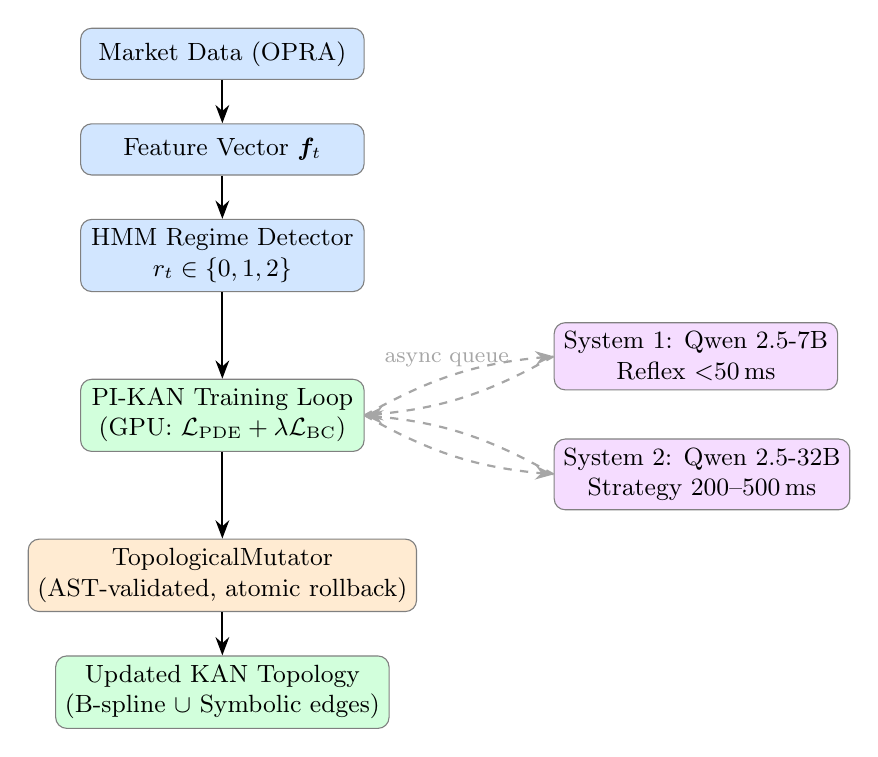
\begin{tikzpicture}[
  node distance=0.55cm and 2.2cm,
  box/.style={rectangle, rounded corners=4pt, draw=black!50, minimum width=3.6cm,
              minimum height=0.65cm, align=center, font=\small},
  databox/.style={box, fill=layerA},
  kannbox/.style={box, fill=layerB},
  agentbox/.style={box, fill=layerC},
  secbox/.style={box, fill=layerD},
  arr/.style={-Stealth, thick},
  dasharr/.style={-Stealth, dashed, thick, gray!70}
]
%% ---- Data column (left) ----
\node[databox] (market)   {Market Data (OPRA)};
\node[databox, below=of market]  (feat)    {Feature Vector $\bm{f}_t$};
\node[databox, below=of feat]    (hmm)     {HMM Regime Detector\\$r_t \in \{0,1,2\}$};

%% ---- PI-KAN (centre) ----
\node[kannbox, below=1.1cm of hmm] (pikan)
  {PI-KAN Training Loop\\(GPU: $\mathcal{L}_\text{PDE}+\lambda\mathcal{L}_\text{BC}$)};

%% ---- Agent (right of PI-KAN) ----
\node[agentbox, right=2.4cm of pikan, yshift= 0.75cm] (sys1)
  {System~1: Qwen 2.5-7B\\Reflex $<$50\,ms};
\node[agentbox, right=2.4cm of pikan, yshift=-0.75cm] (sys2)
  {System~2: Qwen 2.5-32B\\Strategy 200--500\,ms};

%% ---- Security + output ----
\node[secbox,  below=1.1cm of pikan] (mutator)
  {TopologicalMutator\\(AST-validated, atomic rollback)};
\node[kannbox, below=of mutator] (topology)
  {Updated KAN Topology\\(B-spline $\cup$ Symbolic edges)};

%% ---- Arrows ----
\draw[arr] (market)  -- (feat);
\draw[arr] (feat)    -- (hmm);
\draw[arr] (hmm)     -- (pikan);
% async bidirectional queues
\draw[dasharr] (pikan.east) to[bend left=12]
  node[above, font=\footnotesize, pos=0.45]{async queue} (sys1.west);
\draw[dasharr] (pikan.east) to[bend right=12] (sys2.west);
\draw[dasharr] (sys1.west) to[bend left=12] (pikan.east);
\draw[dasharr] (sys2.west) to[bend right=12] (pikan.east);
% downward flow
\draw[arr] (pikan)   -- (mutator);
\draw[arr] (mutator) -- (topology);
\end{tikzpicture}
\caption{OpKAN information flow across three decoupled layers. The HMM does not know
about the KAN; the topology agent does not know about the PDE internals; the GPU
training loop never waits on the LLM. Dashed arrows are asynchronous (bounded queues;
maxsize=1 for inputs, maxsize=32 for outputs). Sustained throughput of 26,300\,smp/sec
is measured during 5-epoch training; 6,506\,smp/sec is from a 50-step cold-start
microbenchmark (see Section~\ref{sec:experiments:headroom}).}
\label{fig:architecture}
\end{figure}

Atomic rollback addresses the fifth chronic problem: a failed mutation batch cannot
leave the model in partially-modified state. All affected edge modules are snapshotted
via \texttt{copy.deepcopy} before applying any mutations; any exception restores all
objects:

\begin{algorithm}
\caption{Atomic Mutation Application with Rollback}
\begin{algorithmic}[1]
\State $\textit{snapshots} \leftarrow \{\}$
\For{each edge $(l, i, j)$ in \textit{mutations}}
    \State $\textit{snapshots}[l,i,j] \leftarrow \texttt{deepcopy}(\texttt{model.layers}[l].\texttt{edges}[i][j])$
\EndFor
\State \textbf{try:}
\For{each mutation $m$ in \textit{mutations}}
    \State \texttt{TopologicalMutator.mutate\_edge}(\texttt{model}, $m$)
\EndFor
\State \textbf{except Exception as} $e$\textbf{:}
\For{each $(l,i,j) \in \textit{snapshots}$}
    \State $\texttt{model.layers}[l].\texttt{edges}[i][j] \leftarrow \textit{snapshots}[l,i,j]$
\EndFor
\State \textbf{log} rollback event with exception $e$
\end{algorithmic}
\end{algorithm}

\texttt{state\_dict} snapshots are insufficient because \texttt{swap\_edge} replaces
entire \texttt{nn.Module} objects; a \texttt{BSplineEdge} state dict cannot be loaded
into a \texttt{C2SymbolicEdge}. We snapshot module objects rather than parameter tensors.

% =====================================================================
\section{Market Regime Conditioning}
\label{sec:regime}
% =====================================================================

\subsection{Hidden Markov Regime Detector}
\label{sec:regime:hmm}

The regime detector fits a Gaussian HMM with diagonal covariance to five time-series
features: log-return $\ell_t$, realized volatility $\hat{\sigma}_t$ (20-bar window,
annualized), implied volatility $\sigma^\text{IV}_t$, IV--RV spread
$\Delta_t = \sigma^\text{IV}_t - \hat{\sigma}_t$, and IV momentum
$\mu^\text{IV}_t = \sigma^\text{IV}_t - \sigma^\text{IV}_{t-1}$.
Walk-forward inference is used to prevent look-ahead bias.

A persistent problem with rolling HMM inference is state label instability: ``state~0''
in window $t$ may map to ``state~1'' in window $t+1$ after a refit. We fix this with
a realized-volatility sorting pass:
\begin{equation}
\pi = \text{argsort}(\bm{\mu}_{:,1}), \quad \text{remap}[s] = \pi^{-1}[s]
\label{eq:hmm_relabel}
\end{equation}
where $\bm{\mu}_{:,1}$ is the vector of per-state mean realized volatilities, ensuring
label~0 always maps to the lowest-volatility regime across all rolling windows.

\subsection{Regime as Topology Signal}
\label{sec:regime:signal}

The HMM regime label feeds System~2's context at every strategic query. A detected
regime transition triggers a strategic request even if fewer than 100 training steps
have elapsed. This is the mechanism by which narrative signals (processed by System~2
into a regime classification) produce structural network adaptation, directly addressing
Problem~4 (regime blindness). Why not let the PI-KAN learn regime-sensitivity directly?
The Heston PDE does not change with regime --- it is a structural prior on the
\emph{shape} of the pricing function. What changes is the parameters
$(\kappa, \sigma, \rho)$. Conflating these two levels would undermine the physics prior.

% =====================================================================
\section{Experimental Evaluation}
\label{sec:experiments}
% =====================================================================

\subsection{Setup}
\label{sec:experiments:setup}

\textbf{Hardware.} NVIDIA H200, CUDA. LLM inference via Ollama (local) with
\texttt{qwen2.5-coder} for protocol benchmarks; vLLM for engineering stress tests.

\textbf{Data.} SLV (silver ETF) option chains with real historical regime features.
Live benchmark: one quote date (cross-sectional split). Replay benchmark: historical
silver/regime feature sequence with replayed SLV surface template.

\textbf{Model families.}
\begin{itemize}[nosep]
  \item \texttt{bs\_plain}: Black-Scholes with baseline ATM volatility.
  \item \texttt{bs\_regime}: Black-Scholes with HMM regime-predicted volatility.
  \item \texttt{rf\_direct}: Random forest direct price prediction.
  \item \texttt{spikan\_hybrid}: Symbolic PI-KAN residual $+$ regime-vol BS anchor.
  \item \texttt{spikan\_plain\_hybrid}: Symbolic PI-KAN residual $+$ plain-formula BS anchor.
  \item \texttt{spikan\_plain\_iv\_hybrid}: Plain-formula anchor $+$ learned IV-space residual (headline hybrid).
\end{itemize}

\subsection{Finding 1: Protocol Validity (RQ1--RQ3)}
\label{sec:experiments:protocol}

\begin{table}[ht]
\centering
\caption{Protocol benchmark results compressed across tiers. Tier~0A: 15 curated
prompts (floor of protocol viability). Tier~0B: 8 document-grounded prompts (primary
evidence tier). Tier~0C/0E: semantic stability and gold agreement (see text).}
\begin{tabular}{@{}lccccc@{}}
\toprule
Context & $n$ & Execute & Intent & Exact DSL & Semantic \\ \midrule
Direct prompt (0A) & 9 & 1.00 & 1.00 & --- & --- \\
Narrative prompt (0A) & 6 & 1.00 & 1.00 & --- & --- \\
Document-grounded (0B) & 8 & 1.00 & 1.00 & --- & --- \\
Paraphrase stability (0C) & 4 grp & --- & --- & 0.75 (grp) & 0.9167 \\
Document-to-gold (0E) & 8 & 1.00 & --- & 0.375 & 0.75 \\ \bottomrule
\end{tabular}
\label{tab:protocol}
\end{table}

The agent correctly compiles analyst intent across all contexts (Execute=1.00 on 0A
and 0B). The semantic agreement of 0.75 on Tiers~0C and~0E reflects a normalization
contract problem: the failing paraphrase group expanded a three-point strike grid to
five points (intent-preserving, structurally different), and regime under-escalation
occurred on one 0E prompt (STRESS compiled as TRANSITION). Neither represents a
comprehension failure. Both are addressable by tighter normalization rules in the
system prompt. The exact agreement ceiling of 0.375 is an open engineering problem,
not an architectural one.

\subsection{Finding 2: Training Objective Insufficiency (RQ4)}
\label{sec:experiments:monotonicity}

\begin{table}[ht]
\centering
\caption{Financial monotonicity checks under explicit DSL regime overrides (Tier~0D).
``Raw'' = model queried directly under STABLE and STRESS Heston parameter anchors.
``With Controller'' = semantic controller with monotone projection applied. All five
checks fail for the raw model; all five pass with the controller.}
\begin{tabular}{@{}lcc@{}}
\toprule
Monotonicity Check & Raw Output & With Controller \\ \midrule
Quote implied vol: STABLE $\to$ STRESS & $\times$ & \checkmark \\
Quote price: STABLE $\to$ STRESS & $\times$ & \checkmark \\
Surface mean vol: STABLE $\to$ STRESS & $\times$ & \checkmark \\
Outlook shock-score: STABLE $\to$ STRESS & $\times$ & \checkmark \\
Shock-risk labels ordered low to high & $\times$ & \checkmark \\
\bottomrule
\end{tabular}
\label{tab:coherence}
\end{table}

This is the central finding. PDE residual minimization is a \emph{necessary but
insufficient} training objective for regime-ordered behavior. The raw model correctly
minimizes $\mathcal{L}_\text{PDE}$; it fails all five monotonicity checks because the
PDE loss imposes no constraint on the ordering of outputs across different Heston
parameter configurations. This is not a deficiency of KANs specifically --- it is a
property of any physics-constrained network trained without explicit regime-ordering
terms in the objective. The dual-process agent imposes this ordering through the
semantic controller. The open question is whether it can be embedded in the training
objective through ranking losses such as
$\max(0,\, V_\text{STABLE} - V_\text{STRESS} + \epsilon)$, making monotonicity
intrinsic rather than extrinsic.

\textbf{Heston parameter anchors.} STABLE: $(\kappa{=}3.0,\,\theta{=}0.02,\,\sigma{=}0.15,\,\rho{=}{-}0.50)$.
STRESS: $(\kappa{=}0.5,\,\theta{=}0.09,\,\sigma{=}0.60,\,\rho{=}{-}0.85)$, with
$r{=}0.05$, $K{=}100$, $T{=}1$. Each model queried at 500 uniformly sampled
$(S,v,t)$ points.

\subsection{Finding 3: Pricing Performance (RQ5)}
\label{sec:experiments:pricing}

\begin{table}[ht]
\centering
\caption{Replay price MAE by market regime. Lower is better.
\texttt{spikan\_plain\_iv\_hybrid} achieves best overall MAE (0.9317), with strength
in transition and stress --- the conditions where regime-conditioned corrections
matter most.}
\begin{tabular}{@{}lcccc@{}}
\toprule
Model & Stable & Transition & Stress & Overall \\ \midrule
\texttt{bs\_plain} & 0.8398 & 2.1037 & 1.6355 & 1.4597 \\
\texttt{spikan\_plain\_hybrid} & 1.1542 & 2.4827 & 0.4745 & 1.3705 \\
\texttt{spikan\_plain\_iv\_hybrid} & 1.1628 & 1.4622 & 0.4239 & \textbf{0.9317} \\
\texttt{rf\_direct} & 8.3183 & 10.2679 & 1.8707 & 6.8190 \\
\bottomrule
\end{tabular}
\label{tab:replay}
\end{table}

\begin{table}[ht]
\centering
\caption{Cross-asset results. The hybrid advantage is consistent on macro-narrative
assets (silver, oil) and absent on structural assets (semiconductors, technology) ---
a domain fit signal, not an architectural failure.}
\begin{tabular}{@{}llcc@{}}
\toprule
Asset & Dominant Signal Type & Best Model & Price MAE \\ \midrule
SLV (silver) & Macro / supply narrative & \texttt{spikan\_plain\_iv\_hybrid} & 0.9317 \\
GLD (gold) & Mean-reverting vol structure & \texttt{bs\_plain} & 1.6515 \\
USO (oil) & Inventory shock / macro & \texttt{spikan\_plain\_iv\_hybrid} & 0.4897 \\
SOXX (semiconductors) & Structural / earnings & \texttt{rf\_direct} & 1.7194 \\
XLK (technology) & Structural / earnings & \texttt{rf\_direct} & 2.5180 \\
\bottomrule
\end{tabular}
\label{tab:cross_asset}
\end{table}

The IV-residual hybrid achieves best overall replay MAE (0.9317). The cross-asset
pattern confirms the architecture's domain specificity: the hybrid wins on silver and
oil (assets where macro narrative and supply-shock interpretation are operationally
relevant), while gold, semiconductor, and technology equities favor simpler baselines.
For SOXX and XLK, the relevant pricing signals (earnings surprise, export controls,
AI capex) are absent from the current feature set --- a signal about where feature
engineering is needed, not a failure of the architecture.

\subsection{Finding 4: Engineering Headroom (RQ6)}
\label{sec:experiments:headroom}

\begin{table}[ht]
\centering
\caption{Engineering performance on NVIDIA H200, batch size 4,096. Sustained
throughput (26,300\,smp/sec) measured during 5-epoch training of 1M rows. The
6,506\,smp/sec E2E microbenchmark reflects cold-start amortization on 50 steps, not
a measurement error.}
\begin{tabular}{@{}lc@{}}
\toprule
Metric & Value \\ \midrule
Sustained training throughput (5 epochs, 1M rows) & 26,300\,smp/sec \\
E2E microbenchmark throughput (50 steps, cold start) & 6,506\,smp/sec \\
System~1 (fast path) latency & $<$50\,ms \\
System~2 (slow path) latency & 200--500\,ms \\
Decision queue overflows (1M-row stress test) & 0 \\
GPU blocking time from LLM & 0\,ms \\
Dual-process vs.\ baseline throughput delta & +4.4\% \\
\bottomrule
\end{tabular}
\label{tab:engineering}
\end{table}

Zero queue overflows and zero GPU blocking validate the non-blocking coordination
design. The +4.4\% throughput advantage over a pure gradient-descent baseline is
likely attributable to System~1's progressive pruning of near-zero edges reducing
the computational graph over time --- a hypothesis requiring ablation. In a
hypothetical synchronous design, a single 500\,ms System~2 decision would block
$\approx 3{,}200$ training steps at sustained throughput; the asynchronous design
reduces this cost to zero.

% =====================================================================
\section{Discussion}
\label{sec:discussion}
% =====================================================================

\subsection{What the Dual-Process Architecture Solves}
\label{sec:discussion:solves}

Each of the five chronic problems maps to a finding. Problems~1 and~5 (stagnation
and $C^2$ instability) are addressed by System~1 reflexive pruning and lr control,
evidenced by zero queue overflows and sustained GPU throughput (Table~\ref{tab:engineering}).
Problems~2, 3, and~4 (parameterization lock-in, symbolic-numerical tension, regime
blindness) are addressed by System~2 strategic surgery, evidenced by all five
monotonicity checks passing only under the controller (Table~\ref{tab:coherence}).

The architecture's key insight is that the cognitive structure of the topology surgery
problem determines the design. These are not two speeds of the same task: they are
qualitatively different cognitive tasks that happen to coexist in the same system.
Forcing them into a single model creates either a bottleneck (if the slow model
handles everything) or incoherence (if the fast model attempts mathematical reasoning).

\subsection{The Training Objective Insufficiency Finding: Generalization}
\label{sec:discussion:generalization}

The monotonicity failure of the raw model generalizes. Any physics-constrained network
trained without regime-ordering terms will fail similar checks under distributional
shift. The PDE loss constrains the solution on the training domain; it does not
enforce behavioral ordering at out-of-distribution query points.

The semantic controller is a structural remedy. The path to making monotonicity
\emph{intrinsic} is enriching the training objective with ranking losses: penalizing
$\max(0,\, V_\text{STABLE} - V_\text{STRESS} + \epsilon)$ on sampled pairs under
the two parameter anchors. MonoKAN \citep{polo_molina_etal_2024_monokan} substitution
on the vol-surface path is a complementary architectural direction. Both remain open.

\subsection{Why This Is Not LangChain}
\label{sec:discussion:notlangchain}

LangChain-style systems route stateless text between API endpoints. Every call is
independent, every output is text, and the system has no persistent mathematical state
to maintain. The dual-process topology agent is qualitatively different along five axes:

\begin{itemize}[nosep]
  \item It manages the \textbf{continuous evolution of a heterogeneous mathematical
  object} (the KAN topology) across thousands of training steps.

  \item Its decisions must satisfy \textbf{formal invariants} ($C^2$, PDE consistency,
  monotonicity) that it reasons about explicitly, not just produce plausible text.

  \item It operates \textbf{concurrently with an ongoing computation} (GPU training
  loop) with non-blocking requirements enforced by bounded queues.

  \item Its actions are \textbf{irreversible without explicit rollback}: a topology
  mutation changes the computational graph --- a \texttt{state\_dict} restore cannot
  undo a parameterization class change from \texttt{BSplineEdge} to
  \texttt{C2SymbolicEdge}.

  \item The two speeds encode \textbf{structurally different cognitive tasks}
  (statistical threshold vs.\ mathematical reasoning), not just different latencies.
\end{itemize}

The closest existing category is not ``LLM tool use'' but \emph{online meta-learning}
--- except the meta-learner here reasons in natural language about mathematical
structure rather than computing a gradient over a meta-objective. The distinction
matters: an LLM that fails to identify a $C^2$-violating symbolic replacement produces
a mathematically broken network, not a grammatically incorrect response.

\subsection{Limitations}
\label{sec:discussion:limitations}

Single quote date for the live benchmark (generalization unestablished). Small protocol
benchmark ($n \leq 15$ per tier). Exact DSL agreement ceiling of 0.375 requires system
prompt engineering. No fine-tuned model weights (LoRA infrastructure exists but
awaits production trajectory data). Monotonicity is still extrinsic to the training
objective. Cross-asset advantage limited to macro-narrative domains.

% =====================================================================
\section{Conclusion}
\label{sec:conclusion}
% =====================================================================

KANs' unique property --- edge-level symbolic replaceability --- creates a topology
surgery problem that gradient descent cannot solve. The dual-process architecture
addresses this problem by matching cognitive task type to model capability: fast
statistical pattern recognition for high-frequency reflexive maintenance (System~1,
7B, $<$50\,ms), slow mathematical reasoning for low-frequency strategic surgery
(System~2, 32B, 200--500\,ms). Demonstrated on a physics-informed KAN under Heston
PDE constraints, the architecture produces regime-ordered behavior that PDE training
alone cannot, with full GPU throughput maintained throughout.

The central finding --- training objective insufficiency --- generalizes beyond options
pricing: any physics-constrained network trained under PDE residuals alone will fail
regime-ordering checks under distributional shift. The semantic controller is a
structural remedy; ranking losses are the path to making monotonicity intrinsic.

The central open problem: can the regime ordering enforced by the semantic controller
be embedded in the training objective through ranking losses, making monotonicity
intrinsic rather than extrinsic? That question, and the five chronic problems of
heterogeneous KAN topology, constitute the research agenda this paper opens.

% =====================================================================
\bibliographystyle{plainnat}
\bibliography{references}

\end{document}
